% GNUPLOT: LaTeX picture with Postscript
\begingroup
  \makeatletter
  \providecommand\color[2][]{%
    \GenericError{(gnuplot) \space\space\space\@spaces}{%
      Package color not loaded in conjunction with
      terminal option `colourtext'%
    }{See the gnuplot documentation for explanation.%
    }{Either use 'blacktext' in gnuplot or load the package
      color.sty in LaTeX.}%
    \renewcommand\color[2][]{}%
  }%
  \providecommand\includegraphics[2][]{%
    \GenericError{(gnuplot) \space\space\space\@spaces}{%
      Package graphicx or graphics not loaded%
    }{See the gnuplot documentation for explanation.%
    }{The gnuplot epslatex terminal needs graphicx.sty or graphics.sty.}%
    \renewcommand\includegraphics[2][]{}%
  }%
  \providecommand\rotatebox[2]{#2}%
  \@ifundefined{ifGPcolor}{%
    \newif\ifGPcolor
    \GPcolortrue
  }{}%
  \@ifundefined{ifGPblacktext}{%
    \newif\ifGPblacktext
    \GPblacktexttrue
  }{}%
  % define a \g@addto@macro without @ in the name:
  \let\gplgaddtomacro\g@addto@macro
  % define empty templates for all commands taking text:
  \gdef\gplbacktext{}%
  \gdef\gplfronttext{}%
  \makeatother
  \ifGPblacktext
    % no textcolor at all
    \def\colorrgb#1{}%
    \def\colorgray#1{}%
  \else
    % gray or color?
    \ifGPcolor
      \def\colorrgb#1{\color[rgb]{#1}}%
      \def\colorgray#1{\color[gray]{#1}}%
      \expandafter\def\csname LTw\endcsname{\color{white}}%
      \expandafter\def\csname LTb\endcsname{\color{black}}%
      \expandafter\def\csname LTa\endcsname{\color{black}}%
      \expandafter\def\csname LT0\endcsname{\color[rgb]{1,0,0}}%
      \expandafter\def\csname LT1\endcsname{\color[rgb]{0,1,0}}%
      \expandafter\def\csname LT2\endcsname{\color[rgb]{0,0,1}}%
      \expandafter\def\csname LT3\endcsname{\color[rgb]{1,0,1}}%
      \expandafter\def\csname LT4\endcsname{\color[rgb]{0,1,1}}%
      \expandafter\def\csname LT5\endcsname{\color[rgb]{1,1,0}}%
      \expandafter\def\csname LT6\endcsname{\color[rgb]{0,0,0}}%
      \expandafter\def\csname LT7\endcsname{\color[rgb]{1,0.3,0}}%
      \expandafter\def\csname LT8\endcsname{\color[rgb]{0.5,0.5,0.5}}%
    \else
      % gray
      \def\colorrgb#1{\color{black}}%
      \def\colorgray#1{\color[gray]{#1}}%
      \expandafter\def\csname LTw\endcsname{\color{white}}%
      \expandafter\def\csname LTb\endcsname{\color{black}}%
      \expandafter\def\csname LTa\endcsname{\color{black}}%
      \expandafter\def\csname LT0\endcsname{\color{black}}%
      \expandafter\def\csname LT1\endcsname{\color{black}}%
      \expandafter\def\csname LT2\endcsname{\color{black}}%
      \expandafter\def\csname LT3\endcsname{\color{black}}%
      \expandafter\def\csname LT4\endcsname{\color{black}}%
      \expandafter\def\csname LT5\endcsname{\color{black}}%
      \expandafter\def\csname LT6\endcsname{\color{black}}%
      \expandafter\def\csname LT7\endcsname{\color{black}}%
      \expandafter\def\csname LT8\endcsname{\color{black}}%
    \fi
  \fi
    \setlength{\unitlength}{0.0500bp}%
    \ifx\gptboxheight\undefined%
      \newlength{\gptboxheight}%
      \newlength{\gptboxwidth}%
      \newsavebox{\gptboxtext}%
    \fi%
    \setlength{\fboxrule}{0.5pt}%
    \setlength{\fboxsep}{1pt}%
\begin{picture}(6760.00,4320.00)%
    \gplgaddtomacro\gplbacktext{%
      \csname LTb\endcsname%
      \put(470,508){\makebox(0,0)[r]{\strut{}$0$}}%
      \csname LTb\endcsname%
      \put(470,925){\makebox(0,0)[r]{\strut{}$5$}}%
      \csname LTb\endcsname%
      \put(470,1342){\makebox(0,0)[r]{\strut{}$10$}}%
      \csname LTb\endcsname%
      \put(470,1758){\makebox(0,0)[r]{\strut{}$15$}}%
      \csname LTb\endcsname%
      \put(470,2175){\makebox(0,0)[r]{\strut{}$20$}}%
      \csname LTb\endcsname%
      \put(470,2592){\makebox(0,0)[r]{\strut{}$25$}}%
      \csname LTb\endcsname%
      \put(470,3009){\makebox(0,0)[r]{\strut{}$30$}}%
      \csname LTb\endcsname%
      \put(470,3425){\makebox(0,0)[r]{\strut{}$35$}}%
      \csname LTb\endcsname%
      \put(470,3842){\makebox(0,0)[r]{\strut{}$40$}}%
      \csname LTb\endcsname%
      \put(973,349){\makebox(0,0){\strut{}$70$}}%
      \csname LTb\endcsname%
      \put(1663,349){\makebox(0,0){\strut{}$80$}}%
      \csname LTb\endcsname%
      \put(2353,349){\makebox(0,0){\strut{}$90$}}%
      \csname LTb\endcsname%
      \put(3043,349){\makebox(0,0){\strut{}$100$}}%
      \csname LTb\endcsname%
      \put(3732,349){\makebox(0,0){\strut{}$110$}}%
      \csname LTb\endcsname%
      \put(4422,349){\makebox(0,0){\strut{}$120$}}%
      \csname LTb\endcsname%
      \put(5112,349){\makebox(0,0){\strut{}$130$}}%
      \csname LTb\endcsname%
      \put(5802,349){\makebox(0,0){\strut{}$140$}}%
      \csname LTb\endcsname%
      \put(6492,349){\makebox(0,0){\strut{}$150$}}%
    }%
    \gplgaddtomacro\gplfronttext{%
      \csname LTb\endcsname%
      \put(123,2175){\rotatebox{-270}{\makebox(0,0){\strut{}Loss \%}}}%
      \csname LTb\endcsname%
      \put(3525,111){\makebox(0,0){\strut{}Frame size (bytes)}}%
      \csname LTb\endcsname%
      \put(3525,4081){\makebox(0,0){\strut{}Losses on duplicate detection}}%
      \csname LTb\endcsname%
      \put(5806,3699){\makebox(0,0)[r]{\strut{}Lost \% ($\lambda$ = 2)}}%
      \csname LTb\endcsname%
      \put(5806,3540){\makebox(0,0)[r]{\strut{}Lost \% ($\lambda$ = 5)}}%
      \csname LTb\endcsname%
      \put(5806,3381){\makebox(0,0)[r]{\strut{}Lost \% ($\lambda$ = 20)}}%
      \csname LTb\endcsname%
      \put(5806,3222){\makebox(0,0)[r]{\strut{}Lost \% ($\lambda$ = 300)}}%
      \csname LTb\endcsname%
      \put(5806,3063){\makebox(0,0)[r]{\strut{}Lost \% ($\lambda$ = 1000)}}%
    }%
    \gplbacktext
    \put(0,0){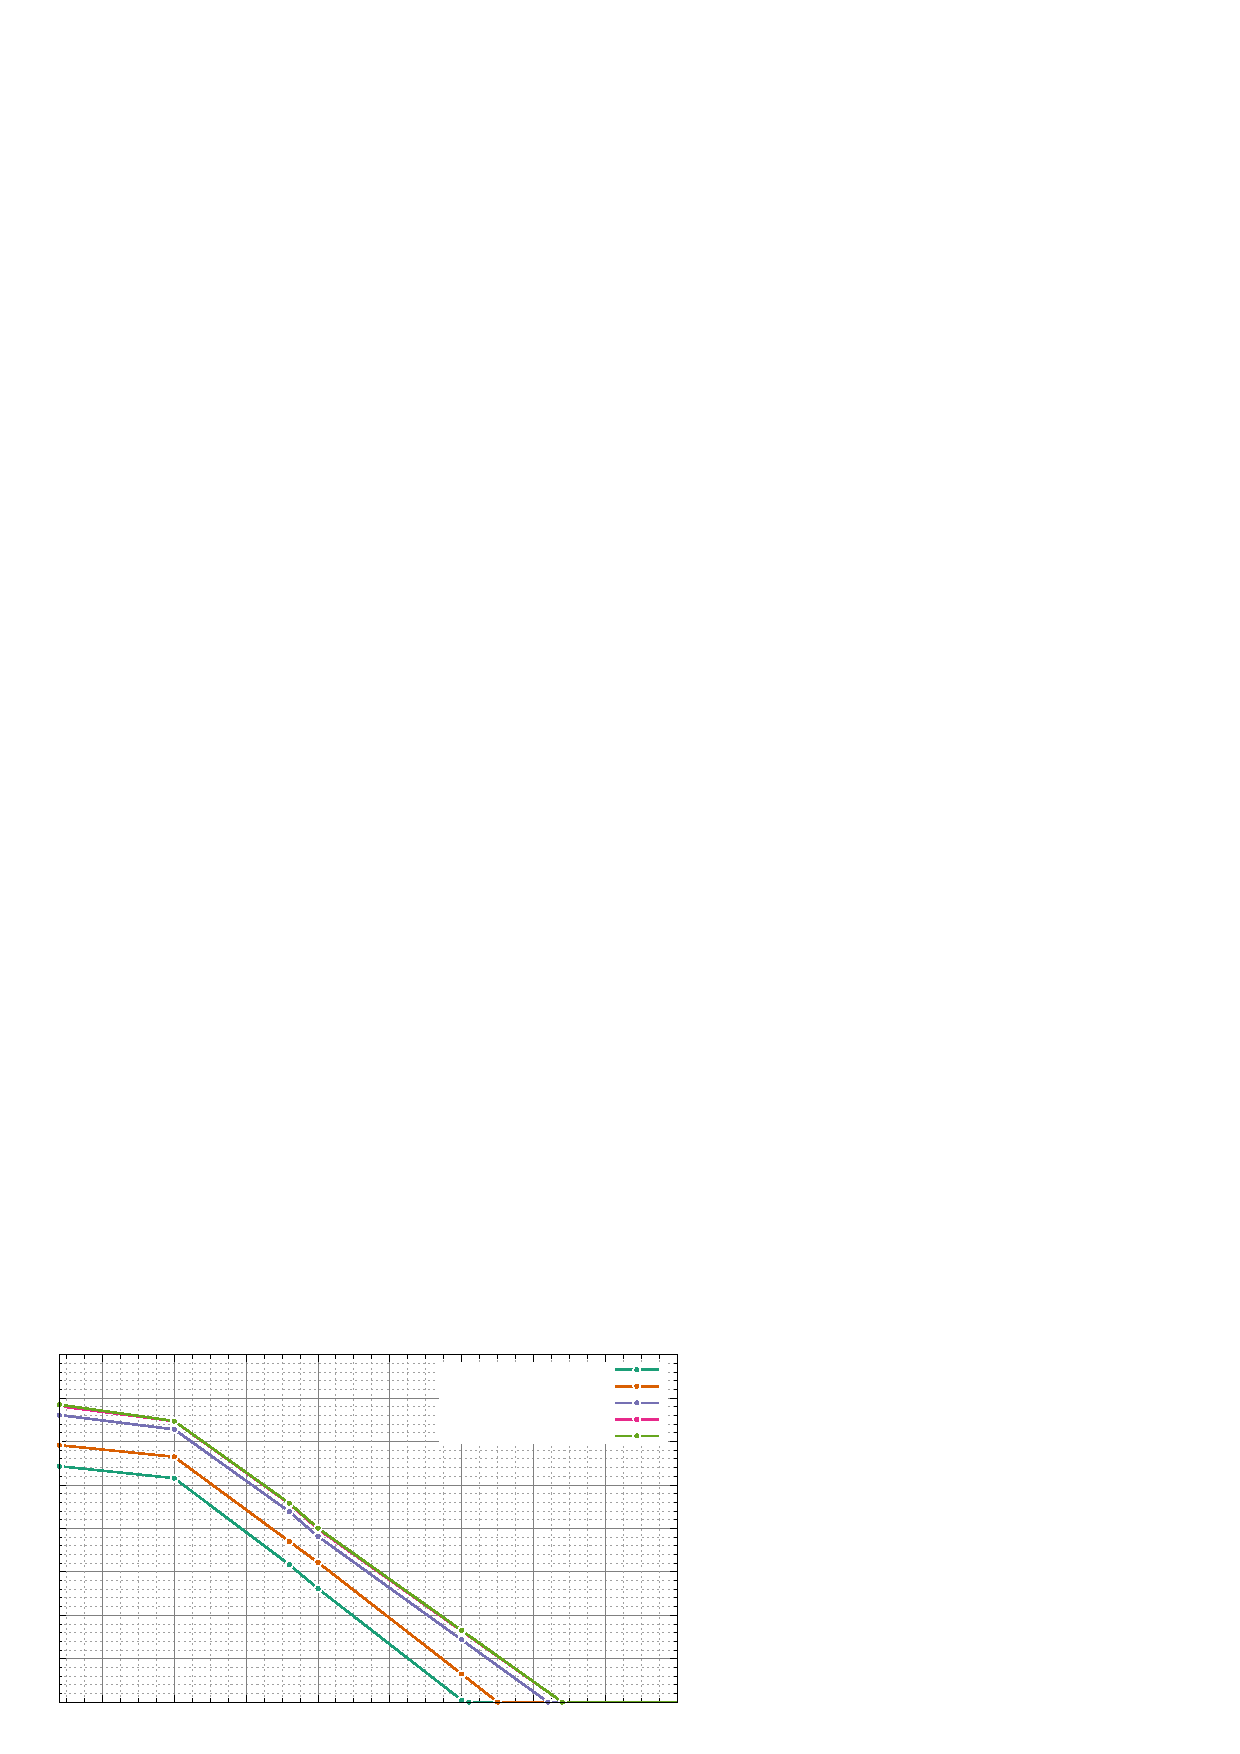
\includegraphics{gnuplot/duplicate-rates}}%
    \gplfronttext
  \end{picture}%
\endgroup
